\def\E{4}
\def\ttau{0.015}
\def\RR{1333.3}
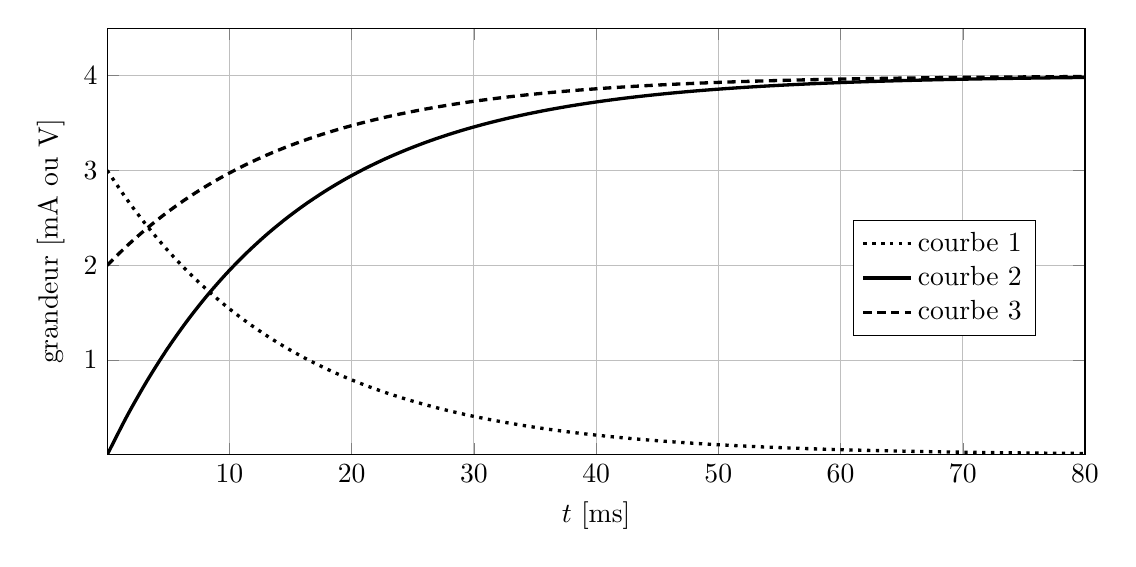
\begin{tikzpicture}[
	trait1/.style={very thick,smooth,samples=50,draw=\JRLblue},
	trait2/.style={very thick,smooth,samples=50,draw=\JRLred},
	trait3/.style={very thick,smooth,samples=50,draw=\JRLorange},
	]
	\begin{axis}[
	xmin=-0,xmax=0.08,
	ymin=0,ymax=4.5,
	width=14cm,height=7cm,
	grid=both,
	ytick={1,2,3,4},
	xtick={.01,.02,.03,.04,.05,.06,.07,.08},
	xticklabels={10,20,30,40,50,60,70,80},
	xlabel={$t$~[ms]},ylabel={grandeur~[mA ou V]},
	ylabel near ticks,
	xlabel near ticks,
	scaled x ticks=false,
	legend style={at={(0.95,0.55)}}
	]
	\addplot[trait1,dotted,domain=0:0.08] {1000*\E / \RR*(exp(-x / \ttau ))}; % *1000 pour avoir des mA
	\addplot[trait2,domain=0:0.08] {\E*(1.0 - exp(-x / \ttau) ) };
    \addplot[trait3,densely dashed,domain=0:0.08] {\E*(1-0.5*exp(-x / \ttau))};
    \legend{courbe $1$,courbe $2$, courbe $3$}
    \end{axis}
\end{tikzpicture}